% ============================================================
% TD : Calcul matriciel
% Pôle Formation UIMM - CVDL - BTS ATI / CRSA - S. JAUBERT
% Travaux dirigés (énoncés). Corrigé : MOD12_Calcul_Matriciel_TD_Corrige_v1_0
% ============================================================
\documentclass[a4paper,11pt]{article}
\usepackage[utf8]{inputenc}
\usepackage[T1]{fontenc}
% babel-french absent sur certains postes : chargement conditionnel
\IfFileExists{french.ldf}{\usepackage[french]{babel}}{}
\usepackage{helvet}
\usepackage{courier}
\renewcommand{\familydefault}{\sfdefault}
\usepackage[top=3cm, bottom=2.5cm, left=2cm, right=2cm, headheight=2cm]{geometry}
\usepackage{amsmath,amssymb,amsfonts}
\usepackage{graphicx}
\usepackage[dvipsnames,table]{xcolor}
\usepackage{tikz}
\usetikzlibrary{arrows.meta, positioning}
\usepackage[most]{tcolorbox}
\usepackage{fancyhdr}
\usepackage{enumitem}
\usepackage{array,needspace}
\usepackage{titlesec}
\usepackage{hyperref}

\definecolor{uimmblue}{HTML}{005C85}
\definecolor{uimmred}{HTML}{D31326}
\definecolor{uimmlightblue}{HTML}{E8F1F8}
\definecolor{uimmgray}{HTML}{333333}
\definecolor{uimmlightgray}{HTML}{F5F5F5}
\hypersetup{colorlinks=true, linkcolor=uimmblue, urlcolor=uimmblue}

\titleformat{\section}{\Large\bfseries\color{uimmblue}}{}{0pt}{}[\vspace{2pt}{\color{uimmblue}\titlerule[1.2pt]}]
\setlist[enumerate,1]{label={\color{uimmblue}\textbf{\arabic*.}}}
\setlist[enumerate,2]{label=\alph*)}
\setlist[itemize,1]{label={\color{uimmblue}\textbullet}}

\newtcolorbox{exo}[1]{colback=white, colframe=uimmblue, fonttitle=\bfseries\color{white},
  coltitle=white, title={#1}, boxrule=1pt, arc=2pt,
  left=8pt, right=8pt, top=5pt, bottom=8pt, before skip=10pt, after skip=8pt, breakable}
\newtcolorbox{consigne}{colback=uimmlightgray, colframe=uimmgray, boxrule=0.8pt, arc=3pt,
  left=8pt, right=8pt, top=6pt, bottom=6pt}

\newcommand{\M}[1]{\begin{pmatrix}#1\end{pmatrix}}
\newcommand{\calc}{\,{\color{uimmred}\small\textbf{[calculatrice]}}}

\pagestyle{fancy}
\fancyhf{}
\renewcommand{\headrulewidth}{0pt}
\fancyhead[L]{\raisebox{-0.5\height}{
\includegraphics[height=1.5cm]{logo_uimm_placeholder.jpg}}}
\fancyhead[C]{\begin{minipage}{8cm}\centering
  {\small\color{uimmblue}\textbf{Pôle Formation UIMM - CVDL}}\\
  {\footnotesize\color{uimmgray} BTS ATI / CRSA -- Mathématiques}\end{minipage}}
\fancyhead[R]{{\small\color{uimmblue}\textbf{MOD12 -- TD}}}
\fancyfoot[C]{{\color{uimmblue}\rule{\textwidth}{1pt}}\\[2pt]
  {\footnotesize\color{uimmgray} Pôle Formation UIMM -- Centre-Val de Loire \hfill S. JAUBERT \hfill \thepage}}

\begin{document}

\begin{tcolorbox}[colback=uimmblue, colframe=uimmblue, sharp corners, boxrule=0pt,
  left=14pt, right=14pt, top=10pt, bottom=10pt]
{\color{white}\LARGE\bfseries Travaux Dirigés -- MOD12}\\[4pt]
{\color{white}\large Calcul matriciel}
\end{tcolorbox}

\vspace{2pt}
\noindent{\small\begin{tabular}{@{}>{\bfseries\color{uimmblue}}l@{\hspace{8pt}}p{13.8cm}@{}}
Période : & Semestre 4 \\
Séquence [S01] : & Matrices et opérations : [C01] écriture matricielle, [C02] calculs, [C03] puissances et processus discrets \\
Séquence [S02] : & Inverse et systèmes : [C01] montrer un inverse, [C02] inverse à la calculatrice, [C03] système par inversion \\
\end{tabular}}

\begin{consigne}
\textbf{Consignes.} Les calculs sur des matrices d'ordre 2 se font \textbf{à la main}, en détaillant. Les questions marquées \calc{} se traitent à la calculatrice : on recopie alors les matrices saisies et le résultat affiché. Chaque résultat se conclut par une phrase avec les unités. Rappels : $(AB)_{ij}$ = ligne $i$ de $A$ $\times$ colonne $j$ de $B$ ; $X_{n+1}=AX_n \Rightarrow X_n = A^nX_0$ ; $AX=B \Rightarrow X = A^{-1}B$.
\end{consigne}

% ============================================================
\needspace{7cm}
\section{Lire et construire une matrice \hfill {\normalsize\color{uimmred}[S01] [C01] [C02]}}

\begin{exo}{Exercice 1 -- Stock de trois entrepôts}
\label{exo:1}
Un distributeur de composants pneumatiques possède trois entrepôts : Orléans, Tours et Bourges. Le stock de quatre références (R1 : vérins, R2 : distributeurs, R3 : régulateurs de pression, R4 : capteurs de position) est donné par la matrice
\[
M = \M{120 & 45 & 0 & 60\\ 80 & 30 & 25 & 40\\ 15 & 60 & 10 & 90}
\qquad
\begin{array}{l}\text{lignes : Orléans, Tours, Bourges}\\ \text{colonnes : R1, R2, R3, R4}\end{array}
\]
\begin{enumerate}[label=\alph*)]
  \item Quel est le format de $M$ ?
  \item Donner $m_{23}$ et $m_{32}$ et traduire chacun par une phrase.
  \item Quel entrepôt ne dispose plus de régulateurs ? Quel coefficient le montre ?
  \item On pose $L = \M{1 & 1 & 1}$. Calculer $LM$ et interpréter le résultat.
  \item On pose $C = \M{1\\1\\1\\1}$. Calculer $MC$ et interpréter le résultat.
\end{enumerate}
\end{exo}

\begin{exo}{Exercice 2 -- Production de deux usines}
\label{exo:2}
Deux usines $U_1$ et $U_2$ fabriquent trois pièces $p_1$, $p_2$, $p_3$. Les productions de janvier et de février sont :
\[
J = \M{500 & 300 & 200\\ 400 & 350 & 150}
\qquad
F = \M{450 & 320 & 180\\ 420 & 330 & 170}
\qquad
\begin{array}{l}\text{lignes : } U_1,\ U_2\\ \text{colonnes : } p_1,\ p_2,\ p_3\end{array}
\]
\begin{enumerate}[label=\alph*)]
  \item Calculer $J+F$ et interpréter.
  \item Calculer $F-J$. Quelle usine a augmenté sa production de $p_1$ ? De combien ?
  \item L'objectif de mars est une hausse de $20\,\%$ par rapport à janvier. Écrire la matrice des objectifs de mars.
  \item Déterminer les réels $a$ et $b$ tels que $\M{2a & 300 & 200\\ 400 & b+50 & 150} = J$.
\end{enumerate}
\end{exo}

% ============================================================
\needspace{7cm}
\section{Produit de matrices \hfill {\normalsize\color{uimmred}[S01] [C02]}}

\begin{exo}{Exercice 3 -- Calculs à la main}
\label{exo:3}
On donne $A = \M{2 & -1\\ 3 & 4}$ et $B = \M{1 & 5\\ -2 & 0}$.
\begin{enumerate}[label=\alph*)]
  \item Calculer $A+B$ et $3A - 2B$.
  \item Calculer $AB$ puis $BA$. Que constate-t-on ?
  \item Calculer $A^2$.
\end{enumerate}
\end{exo}

\begin{exo}{Exercice 4 -- Le bon format}
\label{exo:4}
On considère des matrices $A$ de format $2\times 3$, $B$ de format $3\times 3$, $C$ de format $3\times 1$ et $D$ de format $1\times 2$.\\
Parmi les produits $AB$, $BA$, $AC$, $CA$, $DA$, $AD$, $CD$, $DC$, lesquels existent ? Donner alors leur format.
\end{exo}

\begin{exo}{Exercice 5 -- Chiffre d'affaires et marge}
\label{exo:5}
On reprend la production de janvier de l'exercice 2 : $J = \M{500 & 300 & 200\\ 400 & 350 & 150}$. Les prix de vente unitaires et les coûts de revient unitaires des pièces $p_1$, $p_2$, $p_3$ sont, en euros :
\[
P = \M{8\\12\\20} \qquad\qquad K = \M{5\\7\\13}
\]
\begin{enumerate}[label=\alph*)]
  \item Justifier que le produit $JP$ existe et donner son format. Calculer $JP$ et interpréter.
  \item Calculer $P - K$, puis $J(P-K)$. Que représente ce résultat ?
  \item Les prix augmentent de $5\,\%$. Exprimer le nouveau chiffre d'affaires à l'aide de $JP$ et le calculer.
\end{enumerate}
\end{exo}

\begin{exo}{Exercice 6 -- Plan de charge d'un îlot d'usinage}
\label{exo:6}
Un îlot comprend un tour, une fraiseuse et une rectifieuse. Les temps de passage, en minutes par pièce, pour deux références $A$ et $B$ sont donnés par la gamme
\[
T = \M{12 & 8\\ 15 & 20\\ 5 & 6}
\qquad
\begin{array}{l}\text{lignes : tour, fraiseuse, rectifieuse}\\ \text{colonnes : } A,\ B\end{array}
\]
La commande de la semaine est $X = \M{60\\45}$ ($60$ pièces $A$ et $45$ pièces $B$).
\begin{enumerate}[label=\alph*)]
  \item Calculer $TX$. Que représentent ses coefficients ? Les convertir en heures.
  \item Chaque machine est disponible $35$\,h par semaine. La commande est-elle réalisable ?
  \item Les coûts horaires des machines sont $H = \M{45 & 55 & 60}$ (en €/h). Calculer le coût d'usinage de la commande.
\end{enumerate}
\end{exo}

\begin{exo}{Exercice 7 -- Attention aux habitudes}
\label{exo:7}
\begin{enumerate}[label=\alph*)]
  \item Soient $A = \M{1 & 2\\ 2 & 4}$ et $B = \M{2 & -4\\ -1 & 2}$. Calculer $AB$ et $BA$. Que peut-on dire ?
  \item Soient $C = \M{1 & 1\\ 0 & 1}$ et $D = \M{1 & 0\\ 1 & 1}$. Calculer $(C+D)^2$ puis $C^2 + 2CD + D^2$. Comparer.
  \item Développer $(C+D)^2 = (C+D)(C+D)$ et expliquer l'écart observé en b).
\end{enumerate}
\end{exo}

% ============================================================
\needspace{7cm}
\section{Puissances et processus discrets \hfill {\normalsize\color{uimmred}[S01] [C02] [C03]}}

\begin{exo}{Exercice 8 -- Table tournante d'un robot}
\label{exo:8}
Le plateau d'un poste robotisé tourne de $30^\circ$ à chaque indexation. Dans un repère lié au centre du plateau, une pièce située au point de coordonnées $(x\,;\,y)$ est amenée au point de coordonnées $(x'\,;\,y')$ avec
\[
\M{x'\\y'} = R\M{x\\y}
\qquad\text{où}\qquad
R = \M{\cos 30^\circ & -\sin 30^\circ\\ \sin 30^\circ & \cos 30^\circ} = \M{\frac{\sqrt 3}{2} & -\frac{1}{2}\\[2pt] \frac{1}{2} & \frac{\sqrt 3}{2}}.
\]
\begin{enumerate}[label=\alph*)]
  \item La pièce est au point $(4\,;\,0)$ (en dm). Calculer ses coordonnées exactes après une indexation.
  \item \calc{} Calculer $R^3$. Quelle rotation représente-t-il ? Où se trouve la pièce après trois indexations ?
  \item \calc{} Calculer $R^{12}$ et interpréter.
  \item En déduire, sans calcul, une matrice $S$ telle que $RS = I_2$. Que représente-t-elle pour le plateau ?
\end{enumerate}
\end{exo}

\begin{exo}{Exercice 9 -- Disponibilité d'un parc de machines}
\label{exo:9}
Un atelier exploite $40$ presses. Chaque semaine, une presse est dans l'un des trois états : en marche ($M$), en maintenance préventive ($P$), en panne ($D$). Les relevés de GMAO donnent, d'une semaine à la suivante :
\begin{itemize}
  \item une presse en marche reste en marche avec une probabilité $0{,}85$, part en maintenance préventive avec une probabilité $0{,}10$, tombe en panne avec une probabilité $0{,}05$ ;
  \item une presse en maintenance préventive revient en marche avec une probabilité $0{,}90$ et y reste avec une probabilité $0{,}10$ ;
  \item une presse en panne est remise en marche avec une probabilité $0{,}60$ et reste en panne avec une probabilité $0{,}40$.
\end{itemize}
On note $X_n = \M{m_n\\p_n\\d_n}$ les nombres moyens de presses dans chaque état la semaine $n$. Au départ, $X_0 = \M{40\\0\\0}$.
\begin{enumerate}[label=\alph*)]
  \item Écrire le système donnant $m_{n+1}$, $p_{n+1}$, $d_{n+1}$ en fonction de $m_n$, $p_n$, $d_n$. En déduire la matrice $A$ telle que $X_{n+1} = AX_n$. Vérifier que chaque colonne de $A$ a pour somme $1$ et expliquer pourquoi.
  \item Calculer $X_1$ à la main.
  \item \calc{} Calculer $X_4$, $X_{10}$ et $X_{20}$ (arrondis au centième).
  \item Vers quelle valeur semble tendre la proportion de presses en marche ? Cette proportion s'appelle la disponibilité du parc.
  \item \calc{} Un contrat de maintenance améliore les réparations : une presse en panne est remise en marche avec une probabilité $0{,}80$ (et reste en panne avec une probabilité $0{,}20$). Reprendre la question d). Le gain est-il important ?
\end{enumerate}
\end{exo}

\begin{exo}{Exercice 10 -- Trajets d'AGV}
\label{exo:10}
Des chariots autonomes (AGV) circulent entre quatre zones : Réception ($1$), Stock ($2$), Production ($3$), Expédition ($4$). Les liaisons autorisées, à sens unique, sont les suivantes :
\begin{center}
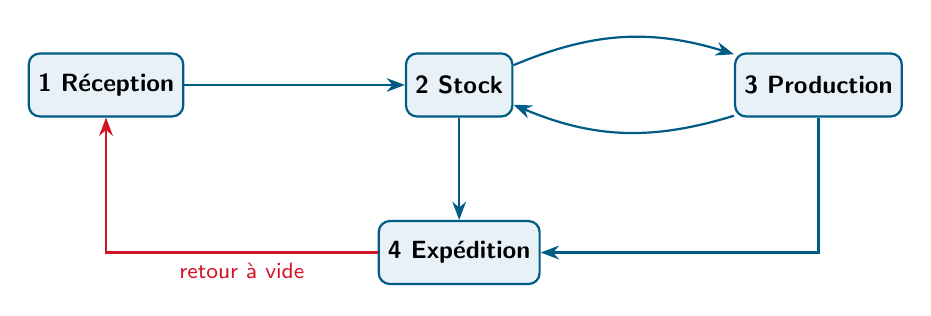
\begin{tikzpicture}[>=Stealth, node distance=2.8cm,
  zone/.style={rectangle, rounded corners, draw=uimmblue, fill=uimmlightblue, thick, minimum size=8mm, font=\bfseries\small}]
  \node[zone] (R) {1 Réception};
  \node[zone, right=of R] (S) {2 Stock};
  \node[zone, right=of S] (P) {3 Production};
  \node[zone, below=1.3cm of S] (E) {4 Expédition};
  \draw[->, thick, uimmblue] (R) -- (S);
  \draw[->, thick, uimmblue] (S) to[bend left=20] (P);
  \draw[->, thick, uimmblue] (P) to[bend left=20] (S);
  \draw[->, thick, uimmblue] (S) -- (E);
  \draw[->, thick, uimmblue] (P) |- (E);
  \draw[->, thick, uimmred] (E) -| node[pos=0.25, below, font=\footnotesize] {retour à vide} (R);
\end{tikzpicture}
\end{center}
On note $G$ la matrice $4\times 4$ telle que $g_{ij} = 1$ s'il existe une liaison de la zone $i$ vers la zone $j$, et $g_{ij} = 0$ sinon.
\begin{enumerate}[label=\alph*)]
  \item Écrire la matrice $G$.
  \item \calc{} Calculer $G^2$ et $G^3$.
  \item On admet que le coefficient $(i,j)$ de $G^k$ donne le nombre de trajets en $k$ étapes de la zone $i$ à la zone $j$. Combien y a-t-il de trajets en $3$ étapes de la réception à l'expédition ? Les écrire.
  \item Combien y a-t-il de trajets en $3$ étapes de la production vers le stock ? Les écrire.
  \item Un AGV peut-il revenir au stock en exactement $2$ étapes ? Justifier avec $G^2$.
\end{enumerate}
\end{exo}

% ============================================================
\needspace{7cm}
\section{Inverse d'une matrice \hfill {\normalsize\color{uimmred}[S02] [C01] [C02]}}

\begin{exo}{Exercice 11 -- Montrer qu'une matrice est l'inverse d'une autre}
\label{exo:11}
\begin{enumerate}[label=\alph*)]
  \item Montrer que $B = \M{3 & -2\\ -4 & 3}$ est l'inverse de $A = \M{3 & 2\\ 4 & 3}$.
  \item En CAO, une translation de vecteur $(2\,;\,0)$ s'écrit en coordonnées homogènes $\M{x'\\y'\\1} = T\M{x\\y\\1}$ avec $T = \M{1 & 0 & 2\\ 0 & 1 & 0\\ 0 & 0 & 1}$. Montrer que $T' = \M{1 & 0 & -2\\ 0 & 1 & 0\\ 0 & 0 & 1}$ est l'inverse de $T$ et interpréter géométriquement.
  \item Soit $C = \M{2 & 4\\ 1 & 2}$. On suppose qu'il existe une matrice $B$ telle que $CB = I_2$. Comparer les lignes de $C$, puis celles de $CB$. Conclure.
\end{enumerate}
\end{exo}

\begin{exo}{Exercice 12 -- Inverse à partir d'une relation}
\label{exo:12}
Soit $A = \M{3 & -2\\ 1 & 0}$.
\begin{enumerate}[label=\alph*)]
  \item Calculer $A^2$ puis $3A - 2I_2$. Que constate-t-on ?
  \item En déduire que $A\times\frac{1}{2}(3I_2 - A) = I_2$.
  \item En déduire que $A$ est inversible et donner $A^{-1}$.
  \item \calc{} Vérifier le résultat à la calculatrice.
\end{enumerate}
\end{exo}

% ============================================================
\needspace{7cm}
\section{Systèmes linéaires \hfill {\normalsize\color{uimmred}[S02] [C02] [C03]}}

\begin{exo}{Exercice 13 -- Saturer un atelier (ordre 2, à la main)}
\label{exo:13}
Un atelier fabrique deux coffrets électriques, $E_1$ et $E_2$. Un coffret $E_1$ demande $3$\,h d'assemblage et $1$\,h de câblage ; un coffret $E_2$ demande $2$\,h d'assemblage et $1$\,h de câblage. Ce mois-ci, on dispose de $240$\,h d'assemblage et de $100$\,h de câblage.
\begin{enumerate}[label=\alph*)]
  \item On note $x$ et $y$ les nombres de coffrets $E_1$ et $E_2$ qui saturent les deux postes. Écrire le système vérifié par $x$ et $y$, puis sa forme matricielle $AX = B$.
  \item Montrer que $A^{-1} = \M{1 & -2\\ -1 & 3}$.
  \item Résoudre le système. Vérifier et conclure.
  \item Le mois suivant, on dispose de $270$\,h d'assemblage et de $110$\,h de câblage. Déterminer la nouvelle production.
\end{enumerate}
\end{exo}

\begin{exo}{Exercice 14 -- Élaboration d'un alliage}
\label{exo:14}
Une fonderie élabore $1\,000$\,kg d'un alliage contenant $610$\,kg de cuivre, $230$\,kg de zinc et $160$\,kg de nickel. Elle dispose de trois lingots de récupération dont les compositions massiques sont :
\begin{center}
\renewcommand{\arraystretch}{1.3}
\begin{tabular}{|l|c|c|c|}
\hline
\rowcolor{uimmlightblue}
 & Lingot $L_1$ & Lingot $L_2$ & Lingot $L_3$ \\
\hline
Cuivre & $70\,\%$ & $50\,\%$ & $60\,\%$ \\
\hline
Zinc & $20\,\%$ & $40\,\%$ & $10\,\%$ \\
\hline
Nickel & $10\,\%$ & $10\,\%$ & $30\,\%$ \\
\hline
\end{tabular}
\end{center}
On note $x$, $y$, $z$ les masses (en kg) de lingots $L_1$, $L_2$, $L_3$ à fondre.
\begin{enumerate}[label=\alph*)]
  \item Écrire le système vérifié par $x$, $y$, $z$ et sa forme matricielle $AX = B$.
  \item \calc{} Déterminer $A^{-1}$ et vérifier que $AA^{-1} = I_3$.
  \item \calc{} Déterminer les masses de chaque lingot. Vérifier que la masse totale est bien de $1\,000$\,kg.
\end{enumerate}
\end{exo}

\begin{exo}{Exercice 15 -- Étalonnage d'un capteur de température}
\label{exo:15}
La tension $U$ (en V) délivrée par un capteur dépend de la température $T$ (en °C). Sur la plage utile, le constructeur propose le modèle $U = aT^2 + bT + c$. Trois mesures d'étalonnage donnent :
\begin{center}
\renewcommand{\arraystretch}{1.3}
\begin{tabular}{|l|c|c|c|}
\hline
\rowcolor{uimmlightblue}
$T$ (°C) & $20$ & $60$ & $100$ \\
\hline
$U$ (V) & $1{,}18$ & $2{,}22$ & $3{,}90$ \\
\hline
\end{tabular}
\end{center}
\begin{enumerate}[label=\alph*)]
  \item Écrire le système de trois équations d'inconnues $a$, $b$, $c$, puis sa forme matricielle.
  \item \calc{} Résoudre le système par inversion.
  \item En déduire la tension attendue à $80$\,°C.
\end{enumerate}
\end{exo}

\begin{exo}{Exercice 16 -- Courants dans un circuit}
\label{exo:16}
L'application des lois de Kirchhoff (loi des nœuds et loi des mailles) à un circuit comprenant trois résistances et deux générateurs conduit au système suivant, où $I_1$, $I_2$, $I_3$ sont des intensités en ampères :
\[
\left\{\begin{array}{rcl} I_1 - I_2 - I_3 &=& 0\\ 20\,I_1 + 40\,I_2 &=& 22\\ 40\,I_2 - 30\,I_3 &=& 6\end{array}\right.
\]
\begin{enumerate}[label=\alph*)]
  \item Écrire ce système sous la forme $AX = B$ (attention aux coefficients nuls).
  \item \calc{} Déterminer $I_1$, $I_2$, $I_3$.
  \item Vérifier le résultat dans la première équation.
\end{enumerate}
\end{exo}

% ============================================================
\needspace{7cm}
\section{Problème de synthèse \hfill {\normalsize\color{uimmred}[S01] [C01] [C02] -- [S02] [C02] [C03]}}

\begin{exo}{Problème -- Les services internes d'une usine}
\label{exo:pb}
Une usine possède deux services internes : Énergie ($E$) et Maintenance ($T$). Chacun travaille pour les ateliers de production mais aussi pour l'autre service et pour lui-même :
\begin{itemize}
  \item pour produire $1$\,k€ d'énergie, le service Énergie consomme $0{,}1$\,k€ d'énergie et $0{,}2$\,k€ de maintenance ;
  \item pour produire $1$\,k€ de maintenance, le service Maintenance consomme $0{,}3$\,k€ d'énergie et $0{,}1$\,k€ de maintenance.
\end{itemize}
Les ateliers de production demandent, pour le trimestre, $135$\,k€ d'énergie et $95$\,k€ de maintenance.\\
On note $x$ et $y$ les productions totales (en k€) des services Énergie et Maintenance.
\begin{enumerate}
  \item \textbf{Mise en équation.}
  \begin{enumerate}
    \item Justifier que $x = 0{,}1x + 0{,}3y + 135$ et écrire l'équation analogue pour $y$.
    \item On pose $X = \M{x\\y}$, $C = \M{0{,}1 & 0{,}3\\ 0{,}2 & 0{,}1}$ et $D = \M{135\\95}$. Montrer que $X = CX + D$, puis que $(I_2 - C)X = D$.
  \end{enumerate}
  \item \textbf{Résolution.}
  \begin{enumerate}
    \item Calculer $I_2 - C$.
    \item \calc{} Déterminer $(I_2 - C)^{-1}$ (on donnera les coefficients sous forme de fractions).
    \item En déduire $x$ et $y$. Interpréter.
  \end{enumerate}
  \item \textbf{Exploitation.}
  \begin{enumerate}
    \item Quelle part de la production d'énergie est consommée par les services eux-mêmes ?
    \item Le trimestre suivant, les ateliers demandent $150$\,k€ d'énergie et $100$\,k€ de maintenance. Déterminer les nouvelles productions sans résoudre à nouveau de système.
  \end{enumerate}
\end{enumerate}
\end{exo}


\end{document}
